%%%%%%%%%%%%%%%%%%%%%%% file template.tex %%%%%%%%%%%%%%%%%%%%%%%%%
%
% This is a general template file for the LaTeX package SVJour3
% for Springer journals.          Springer Heidelberg 2010/09/16
%
% Copy it to a new file with a new name and use it as the basis
% for your article. Delete % signs as needed.
%
% This template includes a few options for different layouts and
% content for various journals. Please consult a previous issue of
% your journal as needed.
%
%%%%%%%%%%%%%%%%%%%%%%%%%%%%%%%%%%%%%%%%%%%%%%%%%%%%%%%%%%%%%%%%%%%
%
% First comes an example EPS file -- just ignore it and
% proceed on the \documentclass line
% your LaTeX will extract the file if required
\begin{filecontents*}{example.eps}
%!PS-Adobe-3.0 EPSF-3.0
%%BoundingBox: 19 19 221 221
%%CreationDate: Mon Sep 29 1997
%%Creator: programmed by hand (JK)
%%EndComments
gsave
newpath
  20 20 moveto
  20 220 lineto
  220 220 lineto
  220 20 lineto
closepath
2 setlinewidth
gsave
  .4 setgray fill
grestore
stroke
grestore
\end{filecontents*}
%
\RequirePackage{fix-cm}
%
%\documentclass{svjour3}                     % onecolumn (standard format)
%\documentclass[smallcondensed]{svjour3}     % onecolumn (ditto)
\documentclass[smallextended]{svjour3}       % onecolumn (second format)
%\documentclass[twocolumn]{svjour3}          % twocolumn
%
\smartqed  % flush right qed marks, e.g. at end of proof
%
\usepackage{graphicx}
\usepackage{amsmath}
\usepackage{amsfonts}
\usepackage{caption}
\usepackage{subcaption}
\captionsetup{compatibility=false}
%
% \usepackage{mathptmx}      % use Times fonts if available on your TeX system
%
% insert here the call for the packages your document requires
%\usepackage{latexsym}
% etc.
%
% please place your own definitions here and don't use \def but
% \newcommand{}{}
%
% Insert the name of "your journal" with
% \journalname{myjournal}
%
\begin{document}

\title{Comparison of Mixed Integer Programming Formulations for the Shared Multicast Tree Problem%\thanks{Grants or other notes
%about the article that should go on the front page should be
%placed here. General acknowledgments should be placed at the end of the article.}
}
\subtitle{Tightening the LP bounds}

%\titlerunning{Short form of title}        % if too long for running head

\author{Dag Haugland        \and
        Marika Ivanova %etc.
}

%\authorrunning{Short form of author list} % if too long for running head

\institute{F. Author \at
              first address \\
              Tel.: +123-45-678910\\
              Fax: +123-45-678910\\
              \email{fauthor@example.com}           %  \\
%             \emph{Present address:} of F. Author  %  if needed
           \and
           S. Author \at
              second address
}

\date{Received: date / Accepted: date}
% The correct dates will be entered by the editor


\maketitle

\begin{abstract}
In this paper we focus on the Shared Multicast Tree problem (SMT), which is 
a task in wireless network design aiming to establish a wireless 
communication network minimizing necessary energy consumption. SMT is a 
generalization of the Shared Broadcast Tree problem (SBT), and can be 
regarded as a Steiner tree problem with a nonlinear objective functinon that
reflects the use in wireless communication. In particular, we consider two 
integer linear programming formulations and investigate how they relate to 
each other. The first model extends the original SMT, while the second one 
is based on a strong formulation of the minimum Steiner tree problem. In 
addition, we present several valid inequalities. Our goal is to achieve a 
stronger LP bound then models studied in previous works, and also to devise 
a method which would allow calculating these lower bounds for instances as 
large as possibe. Numerical experiments suggest that both models are much 
stronger than previous formulations, however, the number of constraints 
makes them impractical for solving instances of even fairly small size as 
the computation takes prohibitively long time. Applying a constraint 
generation scheme on one of the studied models significantly increases the 
size of the instances for which it is possible to calculate a strong LP 
bound. 
\keywords{Wireless communication, broadcast tree, Steiner tree, LP bound, 
valid inequalities}
% \PACS{PACS code1 \and PACS code2 \and more}
% \subclass{MSC code1 \and MSC code2 \and more}
\end{abstract}

\section{Introduction}

\label{intro}

The purpose of a multicast communication in a wireless ad-hoc network is to route information from a sending device to a set of receiving devices. Given a set of wireless devices and distances between them, the task is to assign power to each device, so that the demands of the communication are met and the energy consumption is as low as possible, assuming their locations are fixed. Power efficiency is an important measure in designing ad-hoc wireless networks since the devices typically use batteries as power supply and are therefore heavily energy-constrained. Individual devices work as transceivers, which means that they have the ability to both transmit and receive a signal. Moreover, the power level of a device can be dynamically adjusted during a multicast session.

Unlike wired networks, nodes in ad-hoc wireless networks use omnidirectional antennas, and hence a message reaches all nodes within the communication range of the sender. This range is determined by the power assigned to the sender, which is the maximum rather than the sum of the powers necessary to reach all intended receivers. This feature is often referred to as the wireless multicast advantage \cite{Wieseltier00onthe}. 

A well known and extensively studied task in wireless network design is the Minimum Energy Broadcast (MEB) problem. Given a set of wireless devices with one designated source node among them, the goal is to assign power to individual nodes  which determines their communication ranges inducing a broadcast tree such that a signal initiated by the source reaches all the remaining nodes and the energy consumption for this communication is minimized. Typically, not only one node can act as a source. Every node may initiate a message intended for the remaining nodes. In general, two different sources have two different optimal broadcast trees, which means that the optimal broadcast trees must be calculated separately for every node. Furthermore, in order to route signals correctly, the nodes must be able to recognize which node initiated currently received signal and therefore which broadcast tree is used, or from the relaying device's perspective, which power level should be set. It is obvious that such overhead calculations require additional energy and devices with certain abilities.

The idea of the SBT problem is to maintain a single broadcast tree regardless the source of a signal. Such tree would not be optimal for individual sources, but routing at each node would be considerably simplified. Provided that a single broadcast tree is used, the nodes are no longer required to identify the source of the message in order to set a correct power level. Instead, only the immediate neighbour from which the signal was received must be determined. The objective function in SBT captures not only the power levels of the nodes, but captures also how often a node actually transmits using certain power level. A natural extension of this concept and a forefront of this paper is the Shared Multicast Tree (SMT) problem, in which some of the nodes never initiate any transmission and do not have to receive any signals. They can be used as intermediate forwarding nodes whenever it reduces the resulting power, and thus play the role of Steiner nodes. Devices that can initiate a transmission and also have to receive every message are referred to as \emph{destinations}.

\subsection{Related work}
\subsection{Assumptions and notation}
Formally, an instance of the shared multicast tree problem is a quadruple
$$
\Sigma=(G,D,d,\alpha,c),
$$
where individual components have the following meaning: an ad-hoc wireless network is modeled by a complete graph $G=(V,E)$, where the set $V$ of nodes represents the set of wireless devices and the set of edges $E=\{\{i,j\}:i,j\in V, i\neq j\}$ corresponds to the potential links between them. Often we use the set $A=\{(i,j):i,j\in V,\{i,j\}\in E\}$ that contains all arcs derived from $E$. The set $D\subseteq V$ of \emph{destinations} denotes selected devices that initiate a communication and also are required to receive every message initiated by some other destination. The remaining devices represented by $V\setminus D$ does not have to receive the messages, but can be used as an intermediate nodes and relay a transmission whenever it reduces energy consumption. Next, $d: V\times V\rightarrow \mathbb{R}$ is a function that determines a distance between every two nodes. Constant $\alpha$ is an environmentally dependent parameter typically valued between 2 and 4. Power requirement $p_{ij}$ for sending a message from node $i$ to $j$ is then calculated as $p_{ij}=d^{\alpha}_{ij}$. The task is to find a Steiner tree minimizing given objective function $c$.

If $\{i,j\}$ is an edge in a Steiner tree $T=(V_T,E_T)$ of $G$, we use $T_{i/j}$ to denote the subtree of $T$ consisting of all vertices $k$ such that the path from $k$ to $j$ visits $i$, as introduced in \cite{Haugland12Dual}. Additionally, we define a function $\text{nod}(T_{i/j})$ that returns the number of destinations in $T_{i/j}$. Neighbours of $i$ in $T$ are denoted $i^T_1$, $i^T_2$, $i^T_3, \dots$ in non-increasing order of distance from $i$. If there is no risk of confusion, we simply omit the superscript $T$. The highest and second highest power levels of $i$ are defined by its neighbours $i_1$ and $i_2$, respectively. If $i$ is a leaf, we set $p_{ii_2}=0$.

Let $\mathbf{z} \in \{0,1\}^E$ be a binary vector with components corresponding to edges in $E$. The undirected graph induced by $\mathbf{z}$ is defined as  $G_\mathbf{z}=(V,E_\mathbf{z})$, where $\{i,j\}\in E_\mathbf{z}\Leftrightarrow x_{ij}=1$. The directed graph induced by $\mathbf{x} \in \{0,1\}^A$ is defined analogously. In both cases, the induced (directed) graph is not necessarily connected.  

The reminder of this paper is organized as follows: Section \ref{sec:SBT} describes the SMT problem and gives detailed explanation of its objective function. Integer linear programming formulations, valid inequalities and their analysis are presented in Section \ref{sec:ILP}. Next, results of various numerical experiments are reported in Section \ref{sec:exp}, followed by conclusions in Section \ref{sec:conclusion}.
\section{Shared Broadcast and Multicast Tree problem}
\label{sec:SBT}

A feasible solution to an SMT instance $\Sigma$ is any Steiner tree for given set of destinations $D$ in $G$. Let $T=(V_T, E_T)$ depicted in Fig. \ref{fig:obj} be one such solution. Any node $s\in D$ can initiate a transmission and all the remaining destination must receive it. Let us now consider the node $i$ with three neighbours $i_1$, $i_2$ and $i_3$ ordered by their distance from $i$. If the transmitting node is $a$, $b$ or $i_1$, then the signal reaches $i$ via arc $(i_1,i)$ and all nodes in the subtree $T_{i_1/i}$ denoted by the grey area have already received the signal, and so $i$ does not have to send it back to $i_1$. It suffices if $i$ forwards the signal to the most distant neighbour different than $i_1$, which is in our case $i_2$. By using the power level $p_{ii_2}$ and due to the wireless advantage, the message reaches all the neighbours that have not received it yet. On the other hand, if the transmission is initiated by a destination from $T\setminus T_{i_1i}$ (outside the grey area), then $i$ has to forward it to the most distant neighbour $i_1$, which again causes that all nodes that have not received the signal will be reached.
\begin{figure}[h!]
        \centering
%\label{fig:obj}
        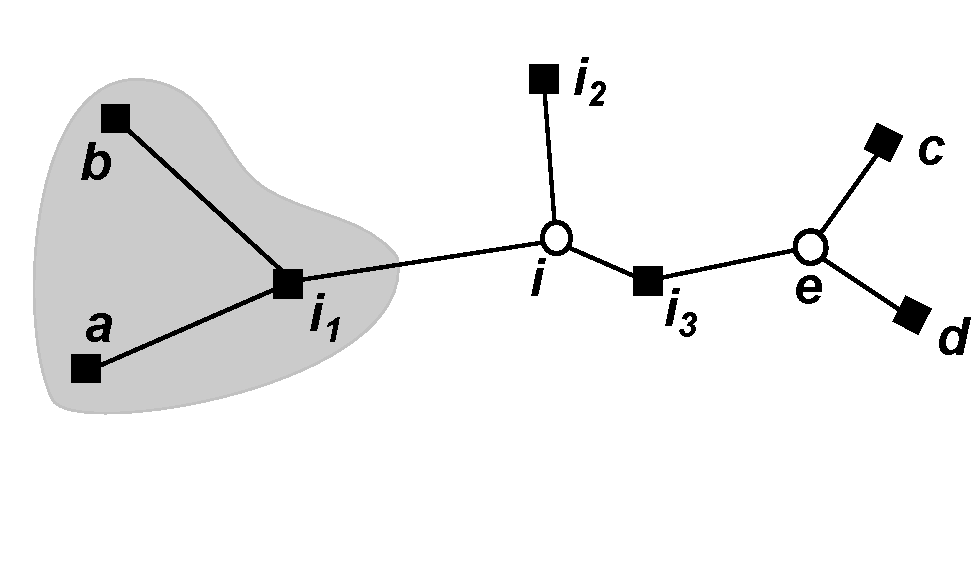
\includegraphics[height=1.6in]{objexp}
        \caption{A simple feasible solution illustrating the calculation of a contribution of node $i$ to the objective function. Destinations and Steiner nodes are denoted by solid squares and empty circles, respectively.}
\end{figure}

 The non-linear objective function captures the entire network structure and takes account of frequency of usage of certain power level. In our example, node $i$ uses the power level $p_{ii_2}$ every time the source of the relayed signal lies in the subtree $T_{i_1/i}$, which contains three potential sources. The power level $P_{ii_1}$ is set whenever the source lies outside of $T_{i_1/i}$, which applies to four sources. The contribution of node $i$ to the objective function is thus $3p_{ii_2} + 4p_{ii_1}$. The total cost of $T$ is the sum over all nodes' contributions. In general,
$$
c(T) = \sum\limits_{i\in V_T}\left[nod(T_{i_1/i})p_{ii_2} + nod(T\setminus T_{i_1/i})p_{ii_2}\right]
$$ 

Like most of the wireless network design problems, SBT/SMT is NP-hard.
\section{MIP Formulations}
\label{sec:ILP}
In this section, we state the known MIP formulation of the shared multicast tree problem and relations between them. Several strengthening valid inequalities are also presented.
\subsection{Original SMT Model}
The first model we consider is slightly improved SMT model introduced in \ref{ref:ivanova}, which contains a weaker version of constraint (\ref{}). This model extends the SBT formulation from \ref{ref:haugland} by the Steiner nodes in order to formulate the multicast version of the problem. The model uses three sets of variables defined as follows:
\newline\newline
  $z_{ij}=
	\begin{cases}
    1 & \text{if edge $\{i,j\} \in E$ is in the solution},\\
    0 & \text{otherwise},
  \end{cases}$
\newline\newline
  $x^{s}_{ij}=
	\begin{cases}
    1 & \text{if arc $(i,j) \in A$ is used to transmit a message from $s\in D$},\\
    0 & \text{otherwise}.
  \end{cases}$
  \newline\newline
  $y^s_{ij}=
	\begin{cases}
    1 & \text{if node $i \in V$ uses power $p_{ij}$ to transmit a message from $s\in D$},\\
    0 & \text{otherwise}.
  \end{cases}$
\newline
\newline    
\begin{subequations}
\begin{flalign}
\label{objective:dd} &\makebox[0pt][l]{$\displaystyle{}\min \sum\limits_{(i,j) \in A} \sum\limits_{s \in D} p_{ij} y^s_{ij} $}  & &&\\ \notag  
\text{s.t.}&  &  &                 && \\	\
\label{con:dd:maxsize}\sum\limits_{\{i,j\}\in E}z_{ij} & \leq  N-1 &  && \\
\label{con:dd:arrowFromDest} \sum\limits_{j\in V_i}x^s_{ji} & = 1 && i,s\in D,i\neq s && \\ 
\label{con:dd:arrowFromNonDestB} \sum\limits_{j\in V_{i}}x^s_{ji} & \leq 1 && i\in V \setminus D, s\in D   &&\\	
\label{con:dd:arrowFromNonDestA} x^s_{ik}  & \leq \sum\limits_{j\in V_{i}\setminus \{k\}}x^s_{ji} && i\in V \setminus D,(i,k)\in A, s\in D   &&\\	
\label{con:dd:extraCon} \sum\limits_{j\in V_{i}}x^s_{ji} & \leq \sum\limits_{j\in V_{i}}x^s_{ij} &&  	i\in V\setminus D, s\in D  &&\\	
\label{con:dd:oneDir} x^s_{ij} + x^s_{ji} & = z_{ij} && \{i,j\}\in E, s\in D &&\\
\label{con:dd:startInSource}  x^i_{ji}    & = 0   &&  i\in D, (j,i)\in A &&\\		 
\label{con:dd:yvar} x^s_{ij} & \leq \sum\limits_{k\in V:p_{ik}\geq p_{ij}}y^s_{ik} && s\in D, (i,j)\in A &&\\  
& \label{con:dd:vardim}	\mathbf{z} \in \{0,1\}^{E}, \mathbf{x},\mathbf{y}\in \{0,1\}^{A\times D} &&	
\end{flalign}~
\end{subequations}   
Let $(\mathbf{x},\mathbf{y}, \mathbf{z})$ be an optimal solution to the SMT model above. Then, the vector $\mathbf{x^s}\in \{0,1\}^{A}$ encapsulates broadcast Steiner arborescences for a source $s\in D$. From $\mathbf{z}\in \{0,1\}^E$ we obtain the resulting (undirected) broadcast Steiner tree. Finally, $\mathbf{y^s}\in \{0,1\}^{A}$ describes the links determining the power levels. The graph induced by $\mathbf{y}$ is  a subgraph of the tree induced by $\mathbf{x}$, and is not necessarily connected.

The number of edges in the resulting Steiner tree is constrained by (\ref{con:dd:maxsize}). Imposing a lower bound $M-1$ on the size of the spanning tree would neither reduce the space of feasible solutions nor increase the strength of the model. If the tree does not contain any Steiner nodes, its size is the lower bound, while if all nodes are used (either as Steiner nodes, or $D = V$), its size equals the upper bound. Constraints (\ref{con:dd:arrowFromDest}) ensures that a message from source $s$ reaches a destination $i$ from exactly one neighbour $j\in V_i$. Analogously, (\ref{con:dd:arrowFromNonDestB}) covers the case when $j \in V\setminus D$: For every source $s$, there is at most one inbound arc to a non-destination $i$. 

If a non-destination $i$ forwards a message from $s$ towards $k$, the message must come from exactly one neighbour $j$ different from $k$, because there is no point in sending the signal backwards. This is ensured by constraint (\ref{con:dd:arrowFromNonDestA}). Note that assuming there is no outgoing arc from a non-destination $j$, (\ref{con:dd:arrowFromNonDestA}) does not prevent $j$ from being a leaf in $G_{\mathbf{x^s}}$. We make such undesired solutions impossible by adding constraint (\ref{con:dd:extraCon}) reducing the set of feasible solutions. However, (\ref{con:dd:extraCon}) is not necessary, because a solution, where a non-destination that does not relay any message is assigned a non-zero power, would be filtered out by optimality. The expression (\ref{con:dd:oneDir}) enforces that an edge $\{i,j\}$ is a part of a solution if and only if for every $s\in D$, either $(i,j)$ or $(i,j)$ is an arc used for sending a message from $s$. The next constraint (\ref{con:dd:startInSource}) expresses that a transmission initiated by $s\in D$ cannot reach $s$ again, which implies non-existence of a directed cycle containing $s$. Finally, by (\ref{con:dd:yvar}), we define a relation between $x$-variables and $y$-variables. When arc $(i,j)$ is used for transmission of a message from $s\in D$, vertex $i$ relaying the message must be assigned power at least $p_{ij}$.
\subsection{$s,t$-Flow Extension}
Consider a network flow problem where one unit of flow must be sent between every pair  $(s,t)$ of destinations. In order to model this requirements, we introduce a variable $f^{st}_{ij}$ as follows:
\newline\newline
  $f_{ij}^{st}=
	\begin{cases}
    1 & \text{if arc $\{i,j\} \in A$ carries 1 unit of flow from $s\in D$ to $t\in D$},\\
    0 & \text{otherwise}.
  \end{cases}$
\newline\newline
The relation between $x$-variables from the original model and $f$-variables is easy to see.
The original SMT formulation can be extended and strengthened by flow constraints for each $(s,t)$-pair.
\newline
\newline    
\begin{subequations}
\begin{flalign}
\label{objective:dd} \makebox[0pt][l]{$\displaystyle{} \min \sum\limits_{(i,j) \in A} \sum\limits_{s \in D} p_{ij} y^s_{ij} $}  \\ 
\text{s.t.}    \notag   \\	
(\ref{objective:dd}),\dots,(\ref{con:dd:yvar}) \notag \\ 
 \label{con:mf:flowNormal}  \sum\limits_{\substack{ j\in V_i}}f^{st}_{ij}-\sum\limits_{\substack{j\in V_i }}f^{st}_{ji}    & = 0   \quad \quad\quad 			  i\in V\setminus\{s,t\}, s,t\in D, s \neq t &\\	
\label{con:mf:flowDest}  \sum\limits_{\substack{ j\in V_t }}f^{st}_{tj}-\sum\limits_{\substack{j\in V_t}}f^{st}_{jt}    & = -1  \quad\quad ~ s,t\in D, s \neq t &\\	
 \label{con:mf:fcap}   f^{st}_{ij} &\leq  x^{s}_{ij},\quad\quad    (i,j)\in A,  s,t\in D, s \neq t  & \\ 		 			 	 
 \label{con:mf:fsym}   f^{st}_{ij} &=  f^{ts}_{ji},  \quad\quad(i,j)\in A,  s,t\in D, s \neq t  &\\   	
\label{con:mf:xydim}	\mathbf{z} \in \{0,1\}^{E}, \mathbf{x},\mathbf{y}\in \{0,1\}^{A\times D}, & \mathbf{f}\in\{0,1\}^{A\times D\times D}. 
\end{flalign}~
\end{subequations}  
The flow conservation constraints (\ref{con:mf:flowNormal})-(\ref{con:mf:flowDest}) guarantee that for each $s,t\in D$ there is a flow of one unit from $s$ to $t$. Next constraint (\ref{con:mf:fcap}) expresses that if an arc $(i,j)$ carries an $s,t$-flow , then this arc is used for sending a message initiated in $s$. The flow symmetry (\ref{con:mf:fsym}) states that arc $(i,j)$ carries a flow from $s$ to $t$ if and only if arc $(j,i)$ carries a flow from $t$ to $s$.

This model can be further extended by valid inequalities strengthening LP bounds
  \begin{subequations}
  \begin{flalign}
\label{con:vi:xImpY}  x^{s}_{ij} & \leq \sum\limits_{t\in D\setminus\{s\}}  f^{st}_{ij},  \quad\quad    (i,j)\in A,s\in D \\
 \label{con:vi:Y1}  \sum\limits_{j\in V\setminus\{s\}}  y^{s}_{sj} & =1,  \quad\quad\quad\quad\quad\quad    s\in D \\
\label{con:vi:f2dest}  f^{st_1}_{ij}-f^{st_2}_{ij}+f^{t_1t_2}_{ij} & \geq 0, \quad\quad\quad\quad\quad\quad i,j \in V,s,t_1,t_2\in D, \\
   &     \notag\quad\quad\quad\quad\quad\quad\quad\quad i\neq j, s\neq t_1,s\neq t_2, t_1\neq t_2  \\
\label{con:vi:sumYImpSumX} \sum\limits_{i\in V\setminus\{j\} }y^{s}_{ji} & \geq \sum\limits_{i\in V\setminus\{j\}}  x^{s}_{ij},   \quad\quad   j\in V\setminus D, s\in D \\
\label{con:vi:sumFImpSumY} \sum\limits_{i\in V\setminus\{j\}, p_{ji}\geq p_{jk}  }f^{st}_{ji} & \leq \sum\limits_{i\in V\setminus\{j\}, p_{ji}\geq p_{jk}}  y^{s}_{ji},   j\in V, s, t\in D, s \neq t, k\in V                     
                      \end{flalign}
  \end{subequations}
\subsection{SMT based on Polzin's Minimum Steiner Tree formulation}

There are many formulations for the Steiner minimum tree problem, that can be a basis for our SMT problem. We consider the formulation $P_{F^2}$, the strongest model studied in \cite{polzin}. The model contains variables
%\newline
%  $y^s_{ij}=
%	\begin{cases}
%    1 & \text{if node $i \in V$ uses power $p_{ij}$ to transmit messages from $s\in D$},\\
%    0 & \text{otherwise}.
%  \end{cases}$
\newline\newline  
  $\check{f}^{st}_{ij}=
	\begin{cases}
    1 & \text{if arc $(i,j) \in A$ carries a flow from the source to both $s,t\in D_1$},\\
    0 & \text{otherwise}.
  \end{cases}$
\newline\newline  
  $f^{t}_{ij}=
	\begin{cases}
    1 & \text{if arc $(i,j) \in A$ carries a flow from the source to $t\in D_1$},\\
    0 & \text{otherwise}.
  \end{cases}$  
\newline\newline  
  $x_{ij}=
	\begin{cases}
    1 & \text{if arc $(i,j) \in A$ is in the solution},\\
    0 & \text{otherwise}.
  \end{cases}$  
\newline
\newline   
The $x$-variables encapsulating the resulting tree correspond to arcs, while analogous $z$-variables in $s,t$-flow model correspond to edges. Hence, an optimal solution obtained by solving the $s,t$-flow model is an undirected tree, and solving $P_{F^2}$ to optimality produces an arborescence rooted in a designated source node $v_0$. Vector $\mathbf{f^s}$ defines a directed path from $v_0$ to $s\in D$ in the arborescence.

We aim to create a SMT model based on Polzin's $P_{F_2}$ model. For this purpose, it is necessary to find a way how to represent the constraint (\ref{con:dd:yvar}) in the Polzin's space. The $y$-variables from the original SMT model have to be used in the extended $P_{F_2}$, because they appear in the objective function which is remains unchanged. By considering the role of individual sets of variables in both models, it is possible to express variables used in one model by variables used in the other model. 
\begin{subequations}
\begin{align}
\label{eq:tr:fstij}f^{st}_{ij}=&f^t_{ij}(1-\check{f}^{st}_{ij})+f^{s}_{ji}(1-\check{f}^{st}_{ji})
&=  f^t_{ij}+f^s_{ji} - \check{f}^{st}_{ij} - \check{f}^{st}_{ji}\\
\label{eq:tr:xijj}x^s_{ij}=&x_{ij}(1-f^{s}_{ij})(1-f^{s}_{ji})+x_{ji}f^{s}_{ji}
&= x_{ij}-f^s_{ij} + f^{s}_{ji} \\
\label{eq:tr:zij}z_{ij}=&&=x_{ij}+x_{ji}
\end{align}
\end{subequations}
Let $T=(V_T,E_T)$ be a multicast tree an consider an edge $\{i,j\}\in E_T$ dividing $T$ into two subtrees $T_i$ and $T_j$ rooted in $i$ and $j$, respectively.  If the arc $(i,j)$ is used for sending a message from $s\in D$ to $t\in D$, then $s$ and $t$ must lie in different subtrees. Node $v_0$ lies either in $T_i$ or $T_j$, as depicted in Fig. \ref{fig:transf_a} and Fig. \ref{fig:transf_b}, respectively. These two cases are captured by the first equality in (\ref{eq:tr:fstij}). If both $v_0$ and $s$ lie in $T_i$, then $f_{ij}^t=1$. Similarly, if $v_0$ and $t$ lie in $T_j$, then $f_{ji}^s=1$. The expressions in parentheses prevent $s$ and $t$ belonging to the same subtree. Further, using the fact that $\check{f^{st}_{ij}}\Rightarrow f_{ij}^t$ and $\check{f^{st}_{ji}}\Rightarrow f_{ji}^s$, we justify the second equality expressing this relation as a linear expression.
\begin{figure*}[h!]
    \centering
    \begin{subfigure}[b]{0.5\textwidth}
        \centering
        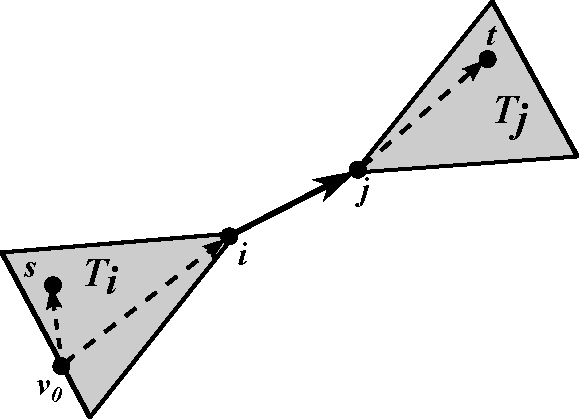
\includegraphics[height=1.2in]{transf_a}
        \caption{Lorem ipsum}
    \end{subfigure}%
    \begin{subfigure}[b]{0.5\textwidth}
        \centering
        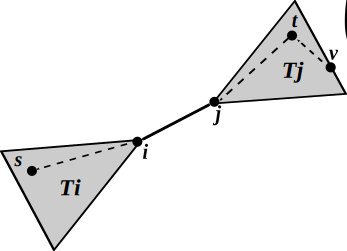
\includegraphics[height=1.2in]{transf_b}
        \caption{Lorem ipsum}
    \end{subfigure}
    \caption{Caption place holder}
\end{figure*}

In the transformation (\ref{eq:tr:xijj}) of $x_{ij}^s$ we distinguish the case when $v_0$ and $s$ are in the same subtree, in which case the arcs $(i,j)$ and $(j,i)$ do not carry a flow to $s$ and when $s$ and $v_0$ belong to different subtrees, and there is a flow via $(j,i)$ towards $s$. Again the last equalities are justified since $f_{ij}^s\Rightarrow x_{ij}$. The relation (\ref{eq:tr:zij}) is obvious.
With these transformations in hand, it is easy to construct a SMT model based on the Steiner minimum tree model $P_{F^2}$:

    \begin{subequations}
    \begin{flalign}
  \min &  \sum\limits_{(i,j) \in A} \sum\limits_{s \in D} p_{ij} y^s_{ij}    \\  \notag  
		   \text{s.t.}&                  && \\	\ 
 \label{con:pf2:flow}  \sum\limits_{\substack{ j \in V_i }}f^{t}_{ji}-\sum\limits_{\substack{j\in V_i}}f^{t}_{ij}    & = \begin{cases}
    1~~~~&  t\in D_1, t = i \\        0~~~~ \qquad             & t\in D_1, i\in V\setminus \{0, t\}\end{cases}     \\	
\label{con:pf2:flowSource}  \sum\limits_{\substack{ j \in V_i }}\check{f}^{st}_{ji}-\sum\limits_{\substack{j\in V_i}}\check{f}^{st}_{ij}    & \geq \begin{cases}
    -1~~~&  s,t\in D_1,s\neq t, i = 0 \\        0  ~~~~   \qquad         & s,t\in D_1,s\neq t, i\in V\setminus \{0\}\end{cases}     \\			
\label{con:pf2:startInSource}  \check{f}^{st}_{ij}    & \leq f^s_{ij}~~   \qquad  \qquad s,t\in D_1,s\neq t, (i,j)\in A \\	
\label{con:pf2:stopInDest}  \check{f}^{st}_{ij}    & \leq f^t_{ij}~~   \qquad    \qquad s,t\in D_1,s\neq t, (i,j)\in A \\			 		
 \label{con:pf2:stronger}  f^{s}_{ij}+f^{t}_{ij}-\check{f}^{st}_{ij}    &\leq x_{ij}    ~~ \qquad \qquad  s,t\in D_1,s\neq t, (i,j)\in A \\			 
		 	 \label{con:pf2:flowX}  \sum\limits_{\substack{ j\in V_i }}x_{ji}-\sum\limits_{\substack{j\in V_i}}x_{ij}    & \leq 0~~~~    \qquad\qquad			  i\in V\setminus D \\			 			   	
		  \label{con:pf2:yvar} x_{ij} -f^s_{ij}+f^s_{ji}  &\leq \sum\limits_{\substack{k\in V: \\ p_{ik}\geq p_{ij}}}y^s_{ik}   ~~\quad  s\in D_1, (i,j)\in A \\  		
\label{con:pf2:B}  \sum_{j\in V_i}x_{ji}&\leq 1~~~~ \qquad  \qquad i\in V\setminus D\\
\label{con:pf2:noflowFromT} f_{ti}^t&=0 ~~~~ \qquad  \qquad t\in D_1, i\in V_t   \\
\label{con:pf2:fitt=xit} f_{it}^t&=x_{it} ~~ \qquad  \qquad t\in D_1, i\in V_t \\
		 			  \label{con:pf2:dim1}  f^s_{ij},\check{f}^{st}_{ij}    & \geq 0    ~~~~ \qquad \qquad	 s,t\in D_1,s\neq t,(i,j)\in A \\			   			  
 \label{con:pf2:dim2}  \mathbf{x}    & \in \{0,1\}^A ,\mathbf{y}  \in \{0,1\}^{A\times D}, \mathbf{f}\in \{0,1\}^{A\times D_1}, \mathbf{\check{f}}\in\{0,1\}^{A\times D_1\times D_1}
    \end{flalign}~
    \end{subequations}
    
    Constraints (\ref{con:pf2:flow})-(\ref{con:pf2:flowX}) formulate the Steiner minimum tree problem. The constraint (\ref{con:pf2:yvar}) has the same purpose as (\ref{con:dd:yvar}), and is expressed in Polzin's space using transformation (\ref{eq:tr:xijj}). By (\ref{con:pf2:B}) we prevent a non-destination from having multiple entering arcs. This is not necessary in the Steiner minimum tree problem formulation, because the objective function causes that such solutions are filtered out by optimization. The necessity of this constraint in SMT is demonstrated in Fig. \ref{fig:Bnecessary}. Similarly, obvious valid inequalities (\ref{con:pf2:noflowFromT}) and (\ref{con:pf2:fitt=xit}) are not necessary in the Steiner minimum tree formulation, but strengthen the SMT model.
\begin{figure}
    \centering
    \begin{subfigure}[b]{0.4\textwidth}
        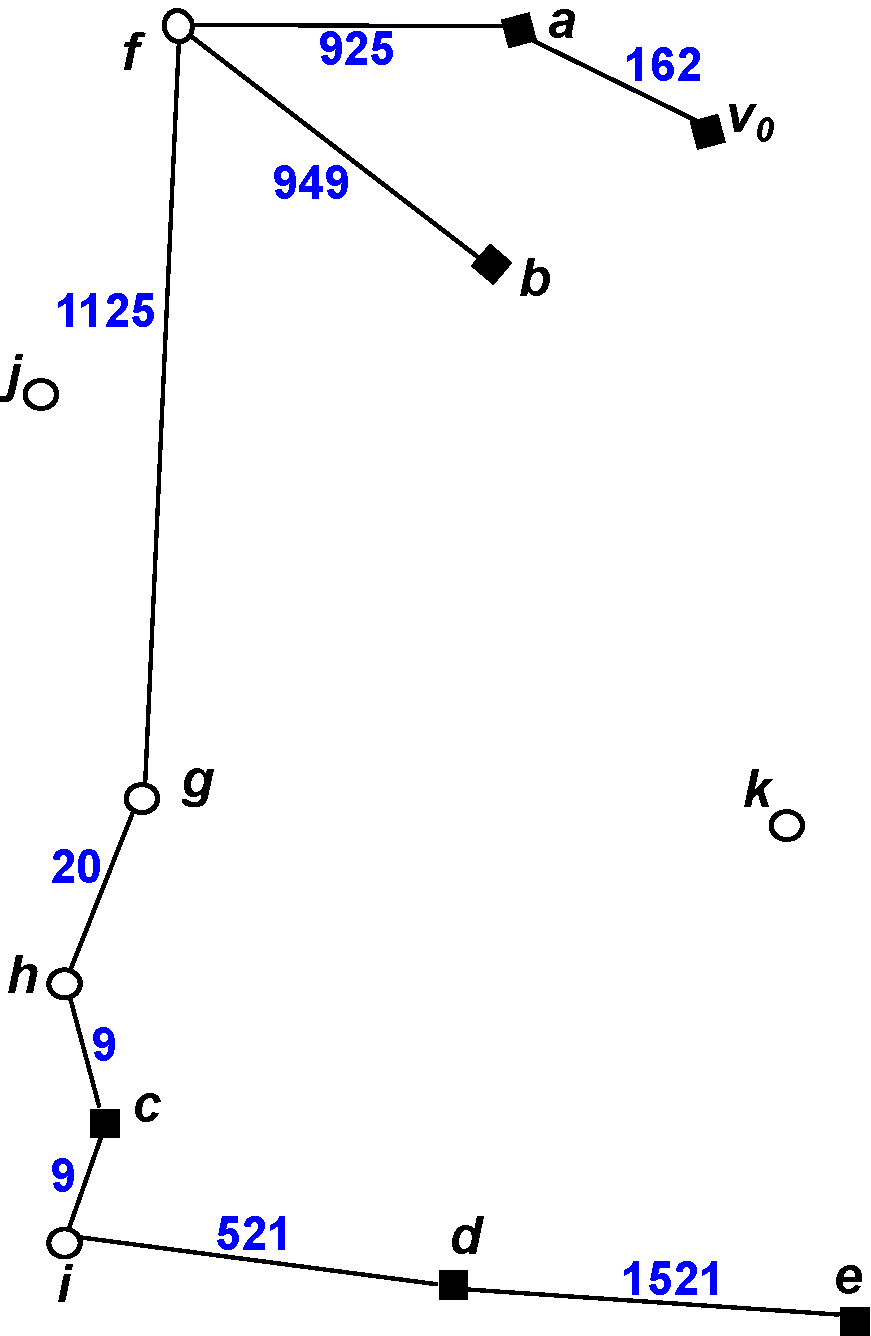
\includegraphics[width=\textwidth]{conBNec}
        \caption{Solution obtained by the original SMT model }
        \label{fig:BorigSMT}
    \end{subfigure}
    \hfill %add desired spacing between images, e. g. ~, \quad, \qquad, \hfill etc. 
      %(or a blank line to force the subfigure onto a new line)
    \begin{subfigure}[b]{0.4\textwidth}
        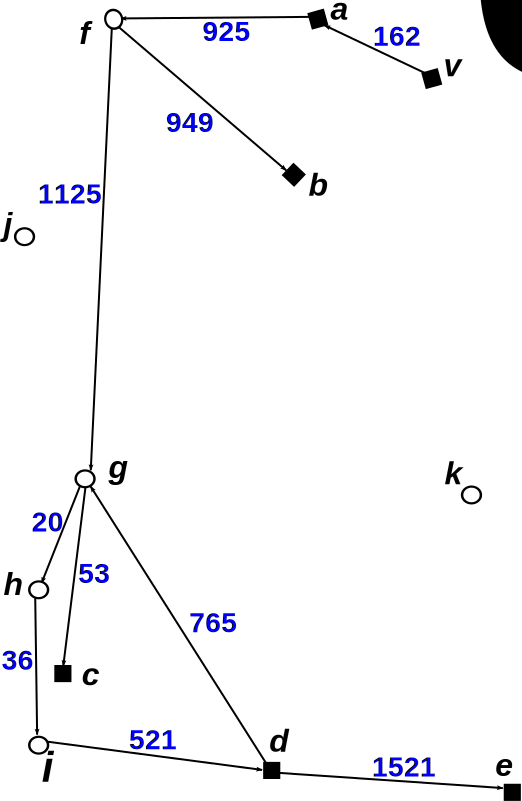
\includegraphics[width=\textwidth]{conBNec2}
        \caption{Solution obtained by Polzin's model without constraint \ref{con:pf2:B}}
        \label{fig:Bpf2}
    \end{subfigure}
    \caption{An exemplary instance showing why the constraint (\ref{con:pf2:B}) is necessary in the SMT model based on Polzin's PF2. Blue numbers denote power requuirements of connection between nodes. For better legibility, the distances of the links are not proportional.}\label{fig:BProof}
\end{figure}    
    
\subsection{Relation between SMT a PF2}
\section{Experimental Evaluation}
\label{sec:exp}
The practical part of this work focuses on comparison of the models presented in the previous section. As the main focus of this study is to determine tighter bounds, the conducted experiments are designed for this purpose. 

\subsection{Constraint generation}
The stronger SMT models are too large and are therefore not very practical as computation of rather smaller instances takes prohibitively long time. That is also the case of the model SMT-MF. The main idea of how to make this model more useful in practice is to dynamically add only those flow constraints that are violated. First, we relax the flow constraints which means that we solve only the LP relaxation of the original SMT model. This gives the vector $\mathbf{x}$, which, by constraint (\ref{smtmf:cap}), acts as a capacity vector, and determines the maximum possible value of a flow through certain arc. Next, we go through all possible $s-t$ pairs of destinations and check whether the flow constraints are fulfilled for the particular $s$ and $t$. New flow constraints for some (possibly all) $s-t$ pairs that violate flow constraints are added to the model and the whole process is repeated until there are no violated flow constraints for any $s-t$ pair. The algorithm \ref{alg:congen} describes this process formally.


There are various strategies how to determine which violated flow constraints will be added to the model. 

\section{Conclusion and Future Work}
\label{sec:conclusion}
as required. Don't forget to give each section
and subsection a unique label (see Sect.~\ref{sec:1}).
%\paragraph{Paragraph headings} Use paragraph headings as needed.
%\begin{equation}
%a^2+b^2=c^2
%\end{equation}

% For one-column wide figures use
%\begin{figure}
% Use the relevant command to insert your figure file.
% For example, with the graphicx package use
%  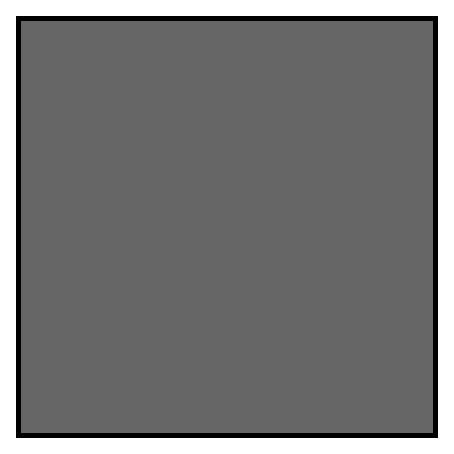
\includegraphics{example.eps}
% figure caption is below the figure
%\caption{Please write your figure caption here}
%\label{fig:1}       % Give a unique label
%\end{figure}
%
% For two-column wide figures use
%\begin{figure*}
% Use the relevant command to insert your figure file.
% For example, with the graphicx package use
%  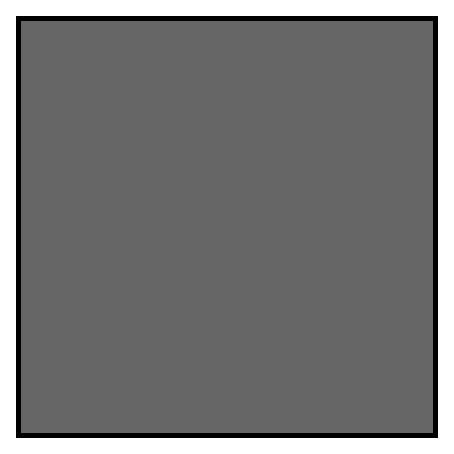
\includegraphics[width=0.75\textwidth]{example.eps}
% figure caption is below the figure
%\caption{Please write your figure caption here}
%\label{fig:2}       % Give a unique label
%\end{figure*}
%
% For tables use
%\begin{table}
% table caption is above the table
%\caption{Please write your table caption here}
%\label{tab:1}       % Give a unique label
% For LaTeX tables use
%\begin{tabular}{lll}
%\hline\noalign{\smallskip}
%first & second & third  \\
%\noalign{\smallskip}\hline\noalign{\smallskip}
%number & number & number \\
%number & number & number \\
%\noalign{\smallskip}\hline
%\end{tabular}
%\end{table}


%\begin{acknowledgements}
%If you'd like to thank anyone, place your comments here
%and remove the percent signs.
%\end{acknowledgements}

% BibTeX users please use one of
%\bibliographystyle{spbasic}      % basic style, author-year citations
%\bibliographystyle{spmpsci}      % mathematics and physical sciences
%\bibliographystyle{spphys}       % APS-like style for physics
%\bibliography{}   % name your BibTeX data base

% Non-BibTeX users please use
\begin{thebibliography}{}
%
% and use \bibitem to create references. Consult the Instructions
% for authors for reference list style.
%
\bibitem{Wieseltier00onthe}
Wieselthier,  J. E., Nguyen, G. D., Ephremides, A.,
On the Construction of Energy-Efficient Broadcast and Multicast Trees in Wireless Networks,
Proceedings of the Nineteenth Annual Joint Conference of the IEEE Computer and Communications Societies.
2, 585--594 (2000)

\bibitem{Haugland12Dual}
Yuan, D., Haugland, D.,
Dual Decomposition for Computational Optimization of Minimum-Power Shared Broadcast Tree in Wireless Networks,
IEEE Transactions on Mobile Computing,
12, 11, 2008--2019 (2012)

\bibitem{Polzin}
Polzin, T., Daneshmand, S. V., A comparison of Steiner tree relaxations, Discrete Applied Mathematics, 112,  1-3, 15 241--261, (2001)
%\bibitem{RefJ}
% Format for Journal Reference
%Author, Article title, Journal, Volume, page numbers (year)
% Format for books
%\bibitem{RefB}
%Author, Book title, page numbers. Publisher, place (year)
% etc
\end{thebibliography}

\end{document}
% end of file template.tex

